\chapter{Treemap Algorithm}

% https://github.com/EduardoVernier/git-latex
% A Stable Greedy Insertion Treemap Algorithm for Software Evolution Visualization

\section{Introduction} \label{sec:intro}
%
%
Understanding the evolution of large and long-lasting software projects is a major aspect of program comprehension. Typically, evolution data for such projects is mined by fact extraction tools from existing software control management systems handing software repositories, such as Git \citep{git}, Subversion \citep{subversion}, and CVS \citep{cvs}.
% I'm not sure how to cite these Source Control Managers, so I'm just linking to their official webpage.
Several types of data attributes are collected (and explored) in this way, including the identity of software items of interest (\emph{e.g.}, packages, folders, files, classes, methods), various quality attributes measured on them (\emph{e.g.}, testability, maintainability, modularity, and readability metrics~\citep{lanza06}), and relations that interrelate these items. \emph{Hierarchy} relations, which describe the containment or aggregation of software items, play a central role in virtually all such evolution analyses, since they offer a powerful and natural way to examine the (typically large) evolution data at multiple levels of detail. As such, methods that can depict time-dependent hierarchies are a central element of the program evolution toolset.

Dynamic, or time-dependent, treemaps are one of the most effective techniques for displaying time-dependent hierarchies. Compared to other techniques, such as node-link tree layouts, they use basically every pixel of the available screen space to display information, and as such scale to tens of thousands of items (tree nodes) per time step. Many treemap methods exist for handling static (time-independent) hierarchies~\citep{shneiderman92,sqr}, which also have been shown to optimize various quality measures that help readability, such as aspect ratio~\citep{sqr, nagamochi07} and relative positions of nodes~\citep{sot,ordered,Ghoniem2015, Buchin2011,nmap}. However, far fewer methods are available for dynamic trees~\citep{hahn10,sondag17,htm}. One key problem for dynamic treemapping is \emph{instability}, \emph{i.e.}, the fact that relatively small changes in a tree can induce disproportionately large changes in the resulting treemaps. Finding a good way to quantify and reduce instability is an open problem for dynamic treemap algorithms.

In this paper, we address the above limitations with two main contributions. Firstly, we propose a new dynamic treemap algorithm, called Greedy Insertion Treemap (GIT). GIT aims to preserve treemap-cell neighborhoods over time by constructing an initial so-called Layout Tree (LT), which is next incrementally updated as the tree data changes, so as to minimize undesired treemap-layout changes.
Secondly, we evaluate the quality of GIT both in the spatial domain and the temporal domain against a large set of well-known treemap algorithms using several established quality metrics, and on a large set of dynamic hierarchies extracted from real-world software repositories. Our evaluation results show that GIT strikes a better balance between spatial and temporal quality than the existing competing methods we evaluated against. As GIT has a simple and computationally scalable implementation, we argue that it represents a valuable contribution to the toolset of techniques needed by program evolution comprehension.

The structure of this paper is as follows. Section~\ref{sec:related_work} outlines existing work on (dynamic) treemapping and related quality metrics, and their use in program evolution comprehension, and also introduces the treemap methods we compare against. Section~\ref{sec:git} details our new GIT algorithm. Section~\ref{sec:evaluation} presents our evaluation methodology for GIT and the obtained results are revealed in Section~\ref{sec:results-3} . Section~\ref{sec:conclusion-3} discusses our proposal and outlines directions for future improvement.


\section{Related Work}
\label{sec:related_work}

In this section, we will discuss the Algorithms (Section~\ref{sec:algorithms}) and Quality Metrics (Section~\ref{sec:metrics-3}) present in the dynamic treemap literature.
Let $T= \{n_i\}$ be a hierarchy (tree) with nodes $n_i$, each having a weight value $a_i \geq 0$. Weights are given for leaf nodes and computed for non-leaf nodes as the sum of their children weights, respectively. Let ${\cal T}(T)$ be the treemap layout of $T$, with a rectangle cell $r_i$ assigned to each $n_i$, so that the area of $r_i$ equals $a_i$.

\subsection{Algorithms}
\label{sec:algorithms}
%
Time-dependent hierarchies $T(t)$ are a central artifact to explore in program evolution comprehension. Since such analyses usually involve tens or even hundreds of time steps $t$, small-multiple visualizations (one image per time step) do not scale well, hence showing an animated layout of the changing hierarchy is preferred~\citep{diehl08}. For this, several techniques construct a so-called union tree $\cup_tT(t)$, build a single layout of this union tree, display it using Icicle plots~\citep{Kruskal1983} or Sunburst diagrams~\citep{sunburst}, and then highlight changes of $T(t)$ over time in it~\citep{ersoy_sequence}. While this approach minimizes instability (layout changes) over time, and is simple to implement, it cannot handle long time sequences and/or large trees.

Treemaps cope well with the need for handling large trees~\citep{schulz11_treesurvey,hci_treemaps,treevis,landesberger11}.  Slice and dice (SND) treemaps introduced the idea but were found to create poor aspect-ratio (AR) cells which are hard to see\,\citep{shneiderman92}. Squarified treemaps (SQR) propose a heuristic that yields good (close to one) AR values\,\citep{sqr}. A subsequent algorithm (APP) was designed to approximate the optimal AR\,\citep{nagamochi07}. While treemaps were originally designed to handle time-independent trees, the need for \emph{stability} was soon revealed -- that is, small changes in the input tree $T$ should yield only small changes in the treemap ${\cal T}(T)$.
Several algorithms were designed to improve stability. Ordered treemaps (OT)~\citep{ordered} and Strip treemaps (STR)~\citep{bederson02} lay out cells $r_i$ using a given order of the nodes of $T$, using different heuristics -- Pivot-by-Middle (PBM), Pivot-by-Size (PBZ), and Pivot-By-Split-Size (PBS)~\citep{ordered}. Other algorithms lay out cells along a space-filling fractal-like curve, \emph{e.g.}, Spiral (SPI)~\citep{spiral}, and Hilbert (HIL) and Moore (MOO) methods~\citep{hilbert_moore}. Yet another ordering technique considers node similarities: Spatially-Ordered Treemaps (SOT)~\citep{sot} processes sibling nodes ordered by decreasing similarity; NMap~\citep{nmap} places cells according to the similarity of their nodes using dimensionality reduction. Variants thereof include NMap Alternate Cuts (NAC), which splits the screen space alternating horizontal and vertical slices; and NMap Equal Weights (NEW) which aims to create similar-size cells.

Stability becomes a major concern when treemapping time-independent trees with potentially long evolution and large variations. However, only a few methods explicitly aim to treat dynamic data. Stable treemaps~\citep{sondag17} aim to improve both AR and stability by using non-sliceable layouts. However, this method is computationally expensive and not trivial to implement. Voronoi treemaps~\citep{balzer05,balzer05b}
achieve, in general, good AR values, and have been adapted to also handle dynamic trees to visualize software structure evolution~\citep{hees17,gotz11}. There exist also methods that propose other cell shapes, or combinations of multiple shapes, such as bubble treemaps~\citep{bubble}, jigsaw treemaps~\citep{jigsaw}, and orthoconvex treemaps~\citep{deberg14}. However, such methods have not been specifically designed with the aim of maximizing stability.
% I believe hybrid was, so I removed it from this list: hybrid treemaps~\citep{htm}


\subsection{Metrics}
\label{sec:metrics-3}
%
As outlined in Sec.~\ref{sec:algorithms}, treemap quality consists of two main components:

\emph{Spatial} quality captures how readable the treemap geometry is. The best known, and most used, metric for this is the aspect ratio (AR) of the cells $r_i$ which should ideally reach one. The so-called readability metric measures how often a user's gaze changes direction while reading an ordered treemap along the predefined node ordering~\citep{bederson02}. The continuity metric measures how often cells of nodes which are close in the given node ordering are far apart in the treemap~\citep{spiral}. % A very similar concept is used to quantify the quality of dimensionality reduction methods~\citep{lamp,martins}. Couldn't find the references...

\noindent\emph{Stability} metrics capture how easily can a user understand the changing geometry of a dynamic treemap. This is measured essentially by quantifying the visual change $\delta(r_i(t), r_i(t+1))$ of the cells $r_i$, and then aggregating such visual changes into a single value using some function $S$. Early on, \cite{ordered} defined the Layout Distance Change metric, where they used for $\delta$ the distance between the vectors $(x_i(t), y_i(t), w_i(t), h_i(t))$ and $(x_i(t+1), y_i(t+1), w_i(t+1), h_i(t+1))$, $x$ and $y$ being the coordinates of the top-left corner, and $w$ and $h$, the width, and the height of a rectangle $r_i$. They defined $S$ as the average of $\delta$ for all cells and revisions. Later, \cite{hahn10} use for $\delta$ the distance between the centers of $r_i(t)$ and $r_i(t+1)$ and also average for $S$. \cite{hilbert_moore} use for $S$ the variance and define $\delta$ as~\citep{ordered}. They also propose a drift metric, which measures how much a cell's center moves away from its average position over long time intervals. Recently, we have seen new metrics that measure stability not by looking only at a single cell's position relative to its past states, but take into consideration the relationships between all cells in the layout. \cite{Hahn2017} propose the relative direction change, which measures angle differences between all centroids in the layout between consecutive time-steps, and \cite{sondag17} propose similar metric, where $\delta$ measures how a cell moves with respect to all its neighbors, where $S$ is again the average.
We will discuss these metrics further, and also propose a new one in Section~\ref{sec:eval_metrics}.

\section{Greedy Insertion Treemap}
\label{sec:git}
%
As outlined in Sec.~\ref{sec:related_work}, many treemapping methods exist in the literature, and these have been evaluated by several metrics for both spatial quality and stability. However, examining the above in more detail, we find two limitations: (a) most existing treemap methods have been designed without the \emph{explicit} aim of maximizing stability; (b) among the few methods where stability was an aim, there is no clear optimal method which yields both good spatial quality and stability for long time sequences of trees exhibiting a high dynamics in terms of node additions, deletions, and weight changes. We next propose a method, Greedy Insertion Treemap (GIT), that aims to outperform the current state-of-the-art in these two respects.


GIT is designed from the start with the aim of increased stability. For this, GIT aims to preserve cell neighborhoods in the treemap over time. To this end, we use a so-called Layout Tree ($LT$) help data structure (not to be confused with the tree $T$ we want to visualize).
Each node $l \in LT$ represents a treemap cell, and may have two subtrees: (a) $R(l)$ is rooted at the top-right corner of $l$; and (b) $B(l)$ is rooted at the bottom-left corner of $l$. Together with the cell weights, $LT$ fully encodes a treemap ${\cal T}$. Indeed, we can construct ${\cal T}$ by traversing $LT$ breadth-first.
During this, for each $l \in LT$, we compute the total weight of its subtrees $R(l)$ and $B(l)$, and cut the remaining drawing space vertically and horizontally according to these summed weights, as illustrated in Fig.~\ref{fig:space-partition}.

\begin{figure}
\centering
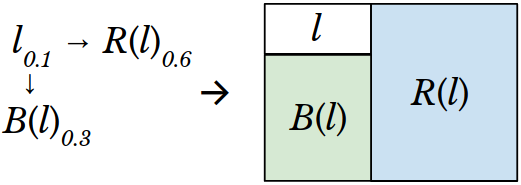
\includegraphics[width=.8\textwidth]{figures/treemap-algorithm/space-partition.png}
\caption{Space partitioning from $LT$.}
\label{fig:space-partition}
\end{figure}

GIT proceeds in two phases: initialization and update, as follows.\\

\noindent\textbf{Initialization:} To start with, we need to construct $LT$ from the first tree $T(t=0)$ in our sequence. For this, we can use basically any method ${\cal T}_{init}$ that constructs a (static) treemap for $T(0)$ from which we can next generate $LT$ with the properties (a) and (b) mentioned above. We have experimented with two such initialization methods. First, we constructed $LT$ from a squarified treemap (\emph{i.e.} ${\cal T}_{init}$ is the SQR algorithm), since SQR is well known to yield very good AR values. Alternatively, we propose a simple heuristic ${\cal T}_{init}^{direct}$ that directly builds $LT$ from the initial tree $T(0)$. Both initialization methods are compared next in Sec.~\ref{sec:results-3}.

To explain our heuristic ${\cal T}_{init}^{direct}$, consider a single-level tree $T = [(n_i,a_i)]  =  [ (A, 10), (B, 2), (C, 8), (D, 4), (E, 1), (F, 3) ]$, to be laid our, for simplicity, in a square drawing area $S$ of size 1; handling general trees is trivial by top-down recursion. We build $LT$ by sequentially adding each $n_i \in T$ to it (Fig.~\ref{fig:git_example}). After each addition, we rebuild ${\cal T}$ from the current $LT$ as explained above, so it covers the entire $S$. Thus, existing nodes are `squeezed' to make space for the new nodes. In our example, we first add node $A$, which will cover the entire $S$. To add $B$, we find the node $n \in LT$ having the worst aspect-ratio cell $c \in {\cal T}$. If $w_c \geq h_c$, we add $B$ directly right of $n$ (as in our example), else we add $B$ directly below $n$, and update ${\cal T}$ from the new $LT$ again. For the third node $C$, as the worst-aspect-ratio cell is $B$, and since $h_B > w_B$, we add $C$ below $B$ and update ${\cal T}$ from $LT$ again. Fig.~\ref{fig:git_example}(d-f) shows the addition of the remaining nodes of $T$.\\

\begin{figure}[htbp!]
\centering

\includegraphics[width=.8\textwidth]{figures/treemap-algorithm/git_example.eps}
\caption{Building the initial layout tree $LT$ (green: inserted cells).}
\label{fig:git_example}
\end{figure}

For didactic purposes, nodes were added in alphabetical order, but in reality, we want nodes to be added in random order, hence when dealing with truly hierarchical data, one sub-tree is not completely laid out before its siblings, which could cause it to be `squeezed'.

\noindent\textbf{Update:} We now have an initial treemap ${\cal T}$ and its $LT$. We next edit $LT$ to handle weight changes, node additions, and node deletions as $T$ changes. \emph{Weight} changes do not change $LT$. \emph{Additions} are handled just as adding regular nodes when building the initial $LT$ using ${\cal T}_{init}^{direct}$. Additions tend to increase the cells' aspect ratios, so we do them after node removals and weight changes. \emph{Removals} are done by editing $LT$ as follows (see also Fig.~\ref{fig:git_removal}):

\begin{enumerate}
\item If a node $n\in LT$ has a $B(n)$ subtree, we replace $n$ by $B(n)$;
\item else if $n$ has a $R(n)$ subtree, we replace $n$ by $R(n)$;
\item else $n$ has no subtrees, so we just remove it from $LT$.
\end{enumerate}

After handling all changes in a new revision of $T$, we rebuild ${\cal T}$ from $LT$, as already explained. As we show next in Sec.~\ref{sec:results-3}, GIT scores a very good balance of spatial quality \emph{vs} stability.

\begin{figure}[htbp!]
\centering
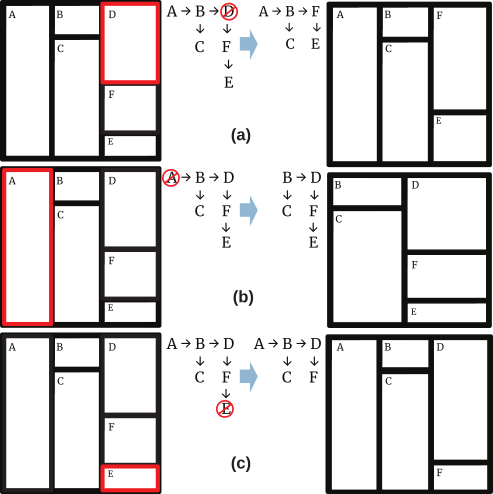
\includegraphics[width=.8\textwidth]{figures/treemap-algorithm/git_removal.eps}
\caption{Removal of nodes (red) from layout tree and its treemap.}
\label{fig:git_removal}
\end{figure}


\section{Evaluation}
\label{sec:evaluation}
%
To evaluate GIT, we considered the following aspects:

\subsection{Metrics}
\label{sec:eval_metrics}
%
To evaluate the quality of GIT, we proceed as follows. For spatial quality, we use the well-known Aspect Ratio metric ($AR$)~\citep{sqr}. For each cell $c$ in a treemap ${\cal T}$, $AR_c = min(w_c, h_c)/max(w_c, h_c)$. This metric is considered by virtually all rectangular treemap evaluations we are aware of.

For stability, we compute three metrics. The first two are the Shneiderman-Wattenberg's Layout Distance Change ($LDC$)~\citep{ordered} and Tak-Cockburn's Location Drift ($LD$)~\citep{hilbert_moore}, already introduced in
Sec.~\ref{sec:related_work}. The $LDC$ metric captures the instability of a cell between consecutive revisions. In contrast, the $LD$ metric captures the deviation of a cell's position over all timesteps.

We also propose a (new) third metric, which extends $LDC$ to also consider the change of the \emph{data}. We define the \emph{visual change} of a cell $c_i$ as the Euclidean distance traveled by the four corners of the rectangle $r_i$ between $t$ and $t+1$, normalized by the treemap diagonal $\sqrt{W^2+H^2}$, so $\delta v_i \in [0,1]$. Next, we define the \emph{data change} of $c_i$ as $\delta a_i = |a_i(t)-a_i(t+1)|$, where $a_i$ is the relative weight of node $c_i$. With these, we define the stability $Q_i$ of a cell $c_i$ in a treemap as

\begin{equation}
Q_i =  (1-\delta v_i) / (1 - \delta a_i).
\label{eqn:stab_ratio}
\end{equation}

We define the stability $Q$ of an entire treemap as the average of its cells' stabilities $Q_i$. In contrast to $LDC$, $Q$ measures how much a rectangle changes \emph{in relation to its data change}. Measuring only absolute changes of rectangles ($LDC$) does not, we believe, fully characterize stability. Indeed, a rectangle could (and should) change a lot if its underlying cell's weight changes a lot. However, this does not mean necessarily that the treemap algorithm is unstable.

\subsection{Techniques}
%
We tested GIT against 14 other treemapping algorithms: Approximate (APP), Hilbert (HIL), Stable treemaps (LM0, LM4), Moore (MOO), NMap-Alternate-Cuts (NAC), NMap-Equal-Weights (NEW), Pivot-by-Middle (PBM), Pivot-by-Size (PBZ), Pivot-by-Split-Size (PBS), Slice- and-Dice (SND), Spiral (SPI), Squarified (SQR), and Strip (STR). For NMap, we use as seed layout the one computed by SQR~\citep{nmap}. We did not consider non-rectangular treemap methods in the evaluation, since not all the metrics in Sec.~\ref{sec:metrics-3} directly generalize to non-rectangular cells.

\subsection{Datasets}
%
We extracted 28 dynamic hierarchies by mining the structure of software projects (folders, files, classes) from 28 corresponding public GitHub repositories, using a custom automated pipeline that scans all available revisions and extracts the code structure using Understand~\citep{understand}. As weights $w_i$, we use the number of lines of code of the respective items. Other software quality metrics delivered by Understand can be used instead, if desired. For more details on this process, we refer to~\citep{vmv}. The considered repositories have quite different sizes, number of revisions, hierarchy depths and shapes, number of developers, and code type (programming languages and application types). Statistics about the datasets are available in Table~\ref{tab:datasets-3}.

\begin{table}[htbp!]
\small
\centering
\scalebox{0.9}{
\begin{tabular}{|l|l|r|r|}
\hline
\textbf{Dataset} & \textbf{Revisions} & \textbf{Nodes (total)} & \textbf{Average depth} \\
\hline
animate.css & 50 & 3454 & 2.87\\
AudioKit & 22 & 11178 & 6.95\\
bdb & 62 & 2658  & 3.83\\
beets & 106   & 9844 & 3.75\\
brackets &  88  & 120292 & 12.85\\
caffe & 44 & 12969   & 4.93\\
calcuta & 50 & 2882 & 10.76\\
cpython   & 321 & 584821 & 6.50\\
earthdata-search   &  46& 18539 & 6.82\\
emcee & 64 & 1746  & 3.62\\
exo & 97 &  36436  & 11.88\\
fsharp   & 69 & 22906 & 7.89\\
gimp   & 72 &  170418 & 5.19\\
hospitalrun-frontend   & 38 &  16759 & 5.71\\
Hystrix & 61 & 15530  & 13.29\\
iina & 74 &  6849  & 4\\
jenkins & 137  & 277185 & 11.94 \\
Leaflet &  84  & 13381 & 4.86 \\
OptiKey   & 36 & 9782 & 6.72\\
osquery  & 37 & 14111 & 5.75 \\
PhysicsJS   & 20 & 2022 & 4.6\\
pybuilder   & 53 & 5457 & 7\\
scikitlearn   & 88 & 48468 & 5.75\\
shellcheck   & 53 & 746 & 2.39\\
soundnode-app   & 35 & 3196 & 6.88\\
spacemacs   & 51 & 10201 & 4.96\\
standard   & 29 & 203 & 2\\
uws & 122 & 4093 & 2.76\\
\hline
\hline
\textbf{Totals:} & 2132 & 1458036 & 5.77\\
\hline
\end{tabular}
}
\caption{Software evolution tree datasets used in the evaluation.}
\label{tab:datasets-3}
\end{table}


\section{Results}
\label{sec:results-3}
%
We evaluate GIT on the aforementioned datasets, algorithms, and metrics collection from several perspectives, by answering a series of questions. Below, average stability $S$ refers to the average of the $LDC$ and $Q$ metrics introduced in Sec.~\ref{sec:metrics-3}. All results that we were not able to fit in the paper can be found at our online repository\citep{git-benchmark}.

\subsection{How does GIT's initialization affect its quality?}
%
As outlined in Sec.~\ref{sec:git}, we can initialize GIT with various treemap layouts, such as squarified (SQR) or using the direct initialization illustrated in Fig.~\ref{fig:git_example}. Intuitively, one would think that SQR initialization is to be preferred, since SQR is well known for its high $AR$ values. To test this, we ran GIT using both initializations for all datasets. After initialization, the same regular GIT update mechanism is used in both cases. Figure~\ref{fig:git_vs_sqr} shows the per-dataset average stability and $AR$ values. Interestingly, we see that the higher-$AR$ SQR initialization actually yields slightly worse $AR$ values for the entire sequence. For stability, the two initializations behave basically identically. We can explain this result by the fact that the GIT direct initialization follows the same heuristics as the update steps, while SQR forces GIT to start with a layout which needs more substantial updates next as the tree data changes. At a higher level, this experiment suggests that GIT performs very well using direct initialization. As such, we use this initialization in all subsequent experiments.

\begin{figure}[htbp!]
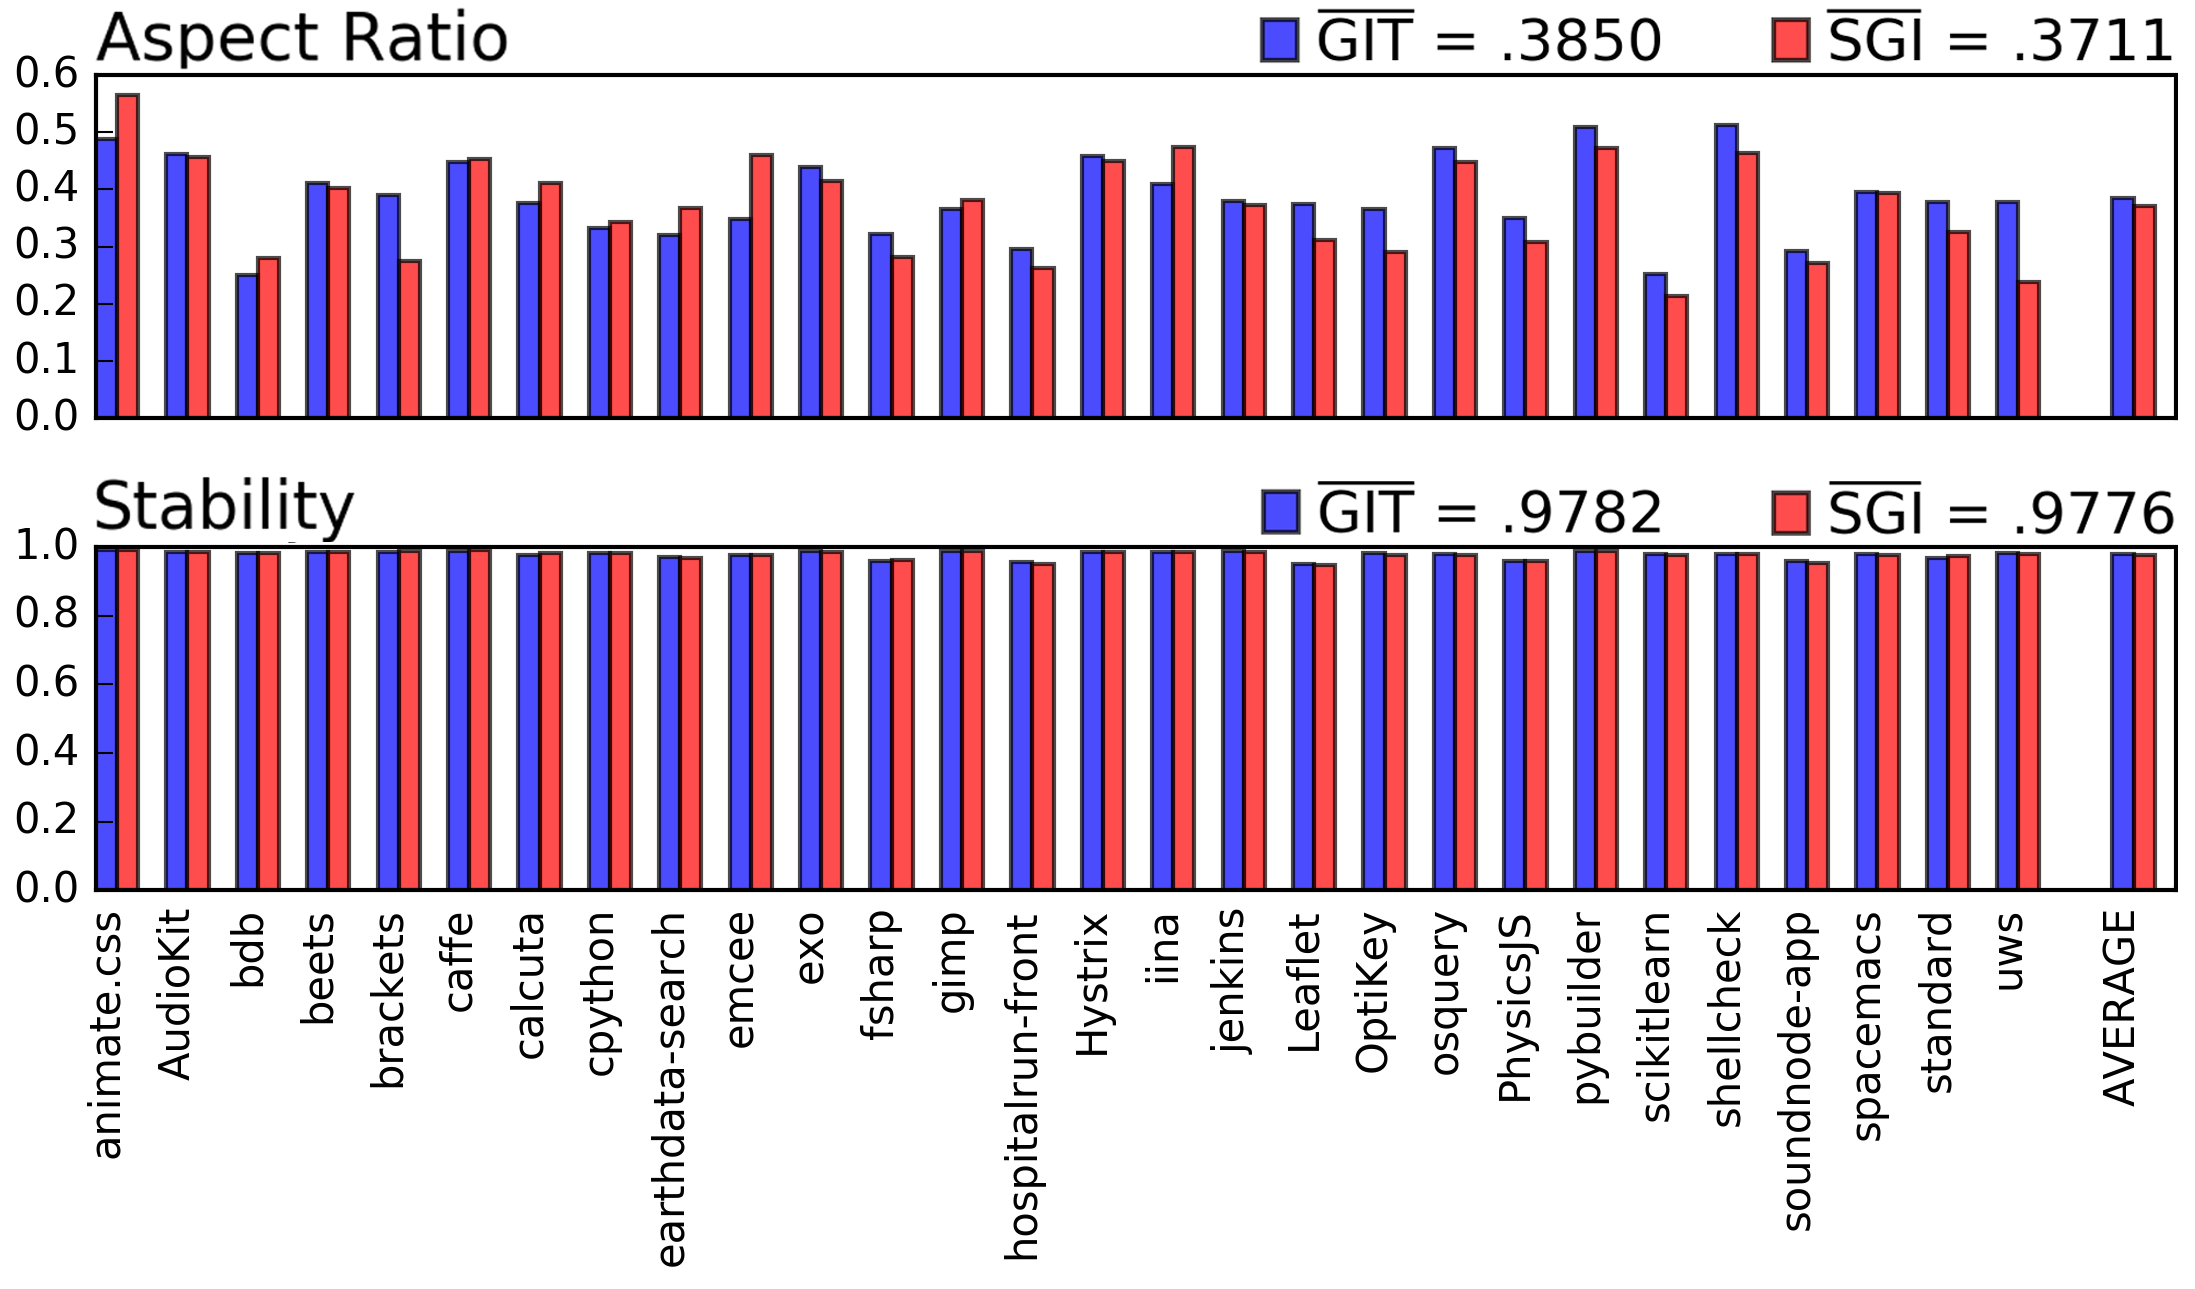
\includegraphics[width=\textwidth]{figures/treemap-algorithm/git-vs-sqrgit-both.png}
\caption{GIT performance using ${\cal T}_{init}^{direct}$ (GIT) \emph{vs} squarified initialization (SGI). }
\label{fig:git_vs_sqr}
\end{figure}

\subsection{How do visual quality and stability vary over time?}
%
As we have already noted, spatial quality and stability are roughly inversely correlated desiderates -- a treemap that scores well for one of these metrics tends to score less well for the other one. Hence, comparing how these metrics change in time is interesting. To answer this, we display, for one dataset and all tested algorithms, two charts showing the median (black), 25-75\% range (green), and 5-95\% range (gray) of the $AR$ and $S$ metrics (Fig.~\ref{fig:boxplots}). We see that APP and SQR have the best $AR$ values, and SND the worst $AR$ values. The other algorithms, including GIT, score in-between. In contrast, GIT, LM0, and SND score the best for stability, while all other algorithms exhibit a non-negligible number of unstable time moments. This suggests that GIT strikes a good compromise between stability and aspect ratio.


\begin{sidewaysfigure}
% \begin{figure*}[htbp!]
\centering
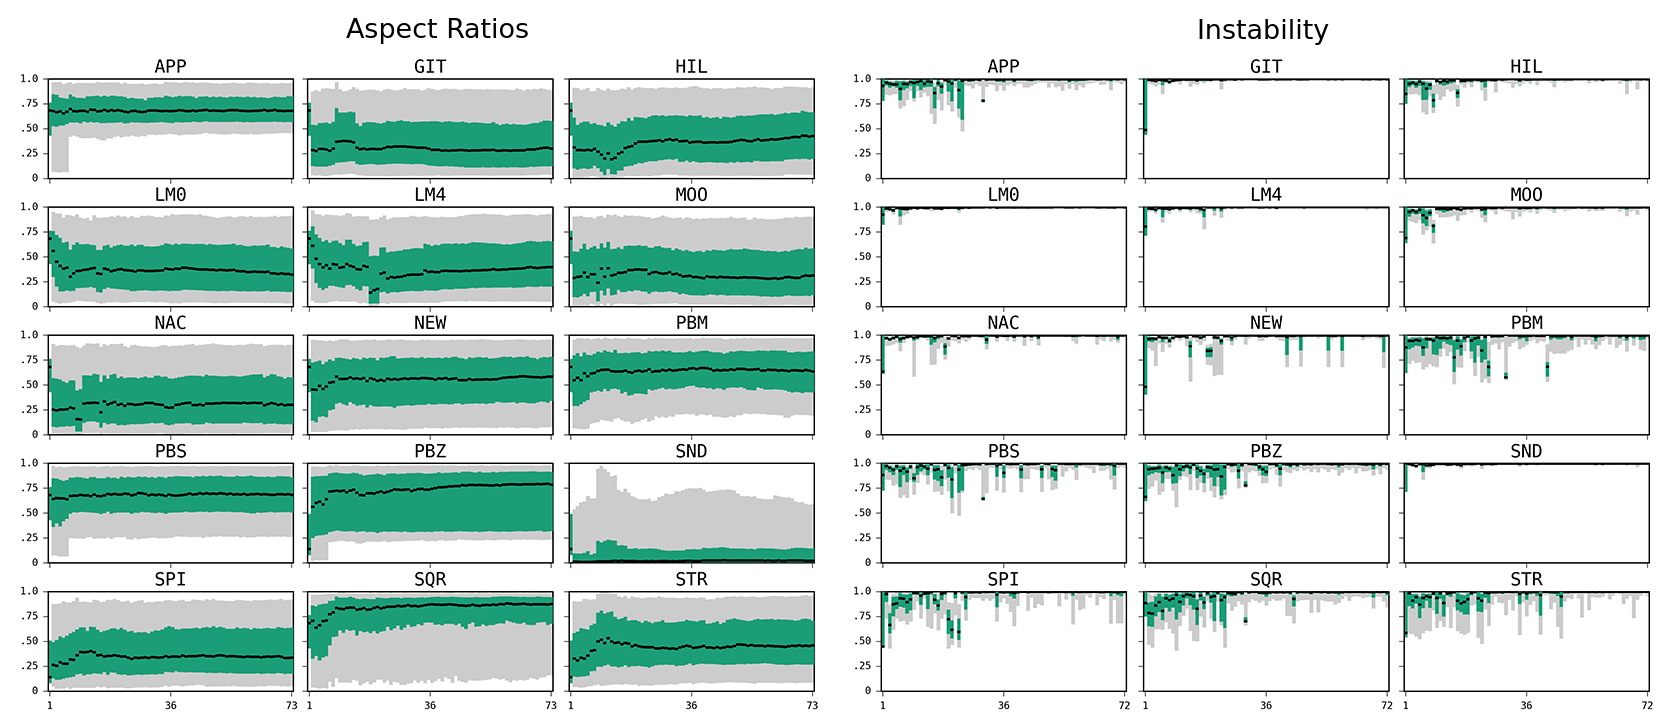
\includegraphics[width=\textwidth]{figures/treemap-algorithm/boxplots-gimp.png}
%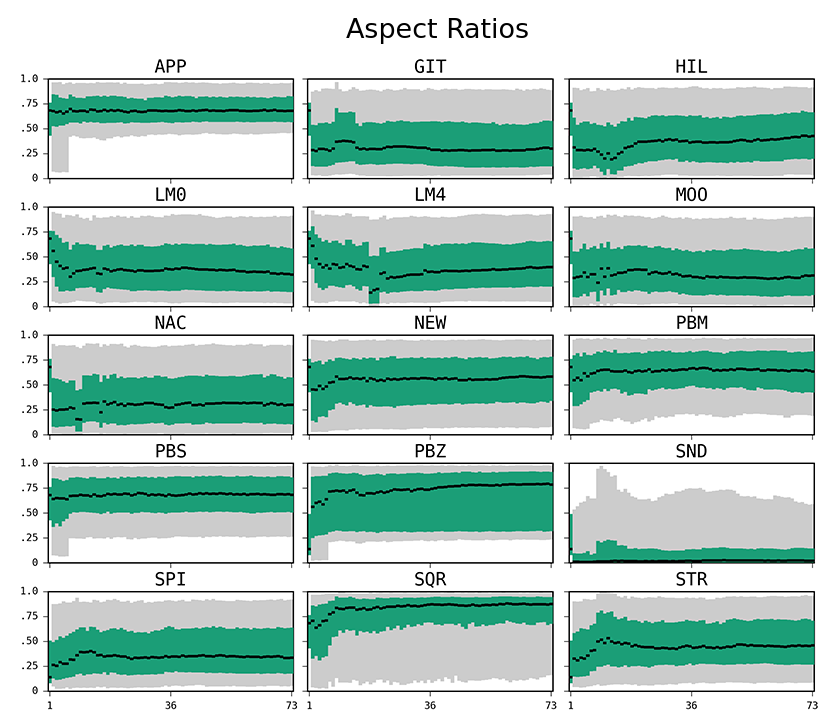
\includegraphics[width=0.69\linewidth]{figures/boxplots-gimp-ar.png}
%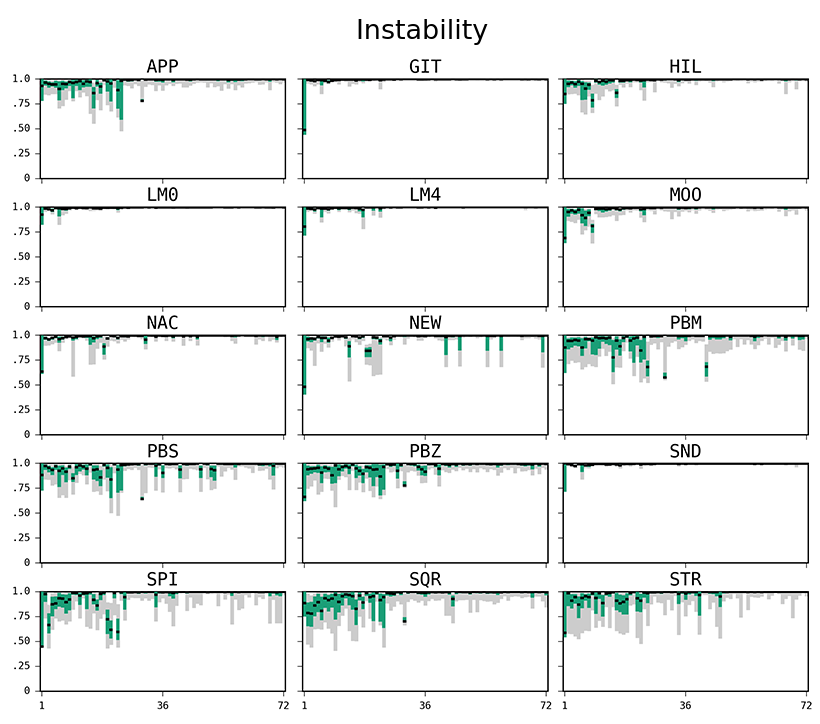
\includegraphics[width=0.69\linewidth]{figures/boxplots-gimp-st.png}
\caption{Distribution of aspect ratio ($AR, left$) and average stability ($S$, right) values over time for the GIMP dataset.}
\label{fig:boxplots}
% \end{figure*}
\end{sidewaysfigure}

While Fig.~\ref{fig:boxplots}(right) shows how the per-timestep stability changes over time, it does not show us which actual instability patterns each method is prone to deliver. Knowing this is useful, as we can better understand what to expect in terms of (undesired) cell moves from a certain algorithm, including GIT. To show this, we plot the trails connecting all centers $k_i(t)$ of all rectangles $r_i(t)$ for consecutive $t$ values over a given tree sequence (Fig.~\ref{fig:centroids}). We set the opacity of each line segment $(r_i(t), r_i(t+1))$ to the Euclidean distance $\| k_i(t) - k_i(t+1)\|$ normalized by the square root of the number of time steps. Hence, dark long lines show big moves (instability) while small moves (close to stability) are hardly visible. The image confirms the high stability of GIT --  in contrast to most other methods, except SND, GIT creates smaller cell moves (shorter dark lines), and most of these are close to horizontal or vertical. Interestingly, we see that other methods create quite different move patterns: SQR, PBS, PBZ, and PBM have mostly (large) diagonal moves. SPI shows a coil-like movement and in STR we see no vertical travel. Overall, we see that GIT is more stable not only because it yields smaller moves, but also because it constrains these to fewer motion directions, thus causes less complex dynamics (that the user must follow) in the resulting visualization. This can be also checked by watching the actual videos showing the algorithms in action~\citep{git-benchmark}.

\begin{figure*}[htbp!]
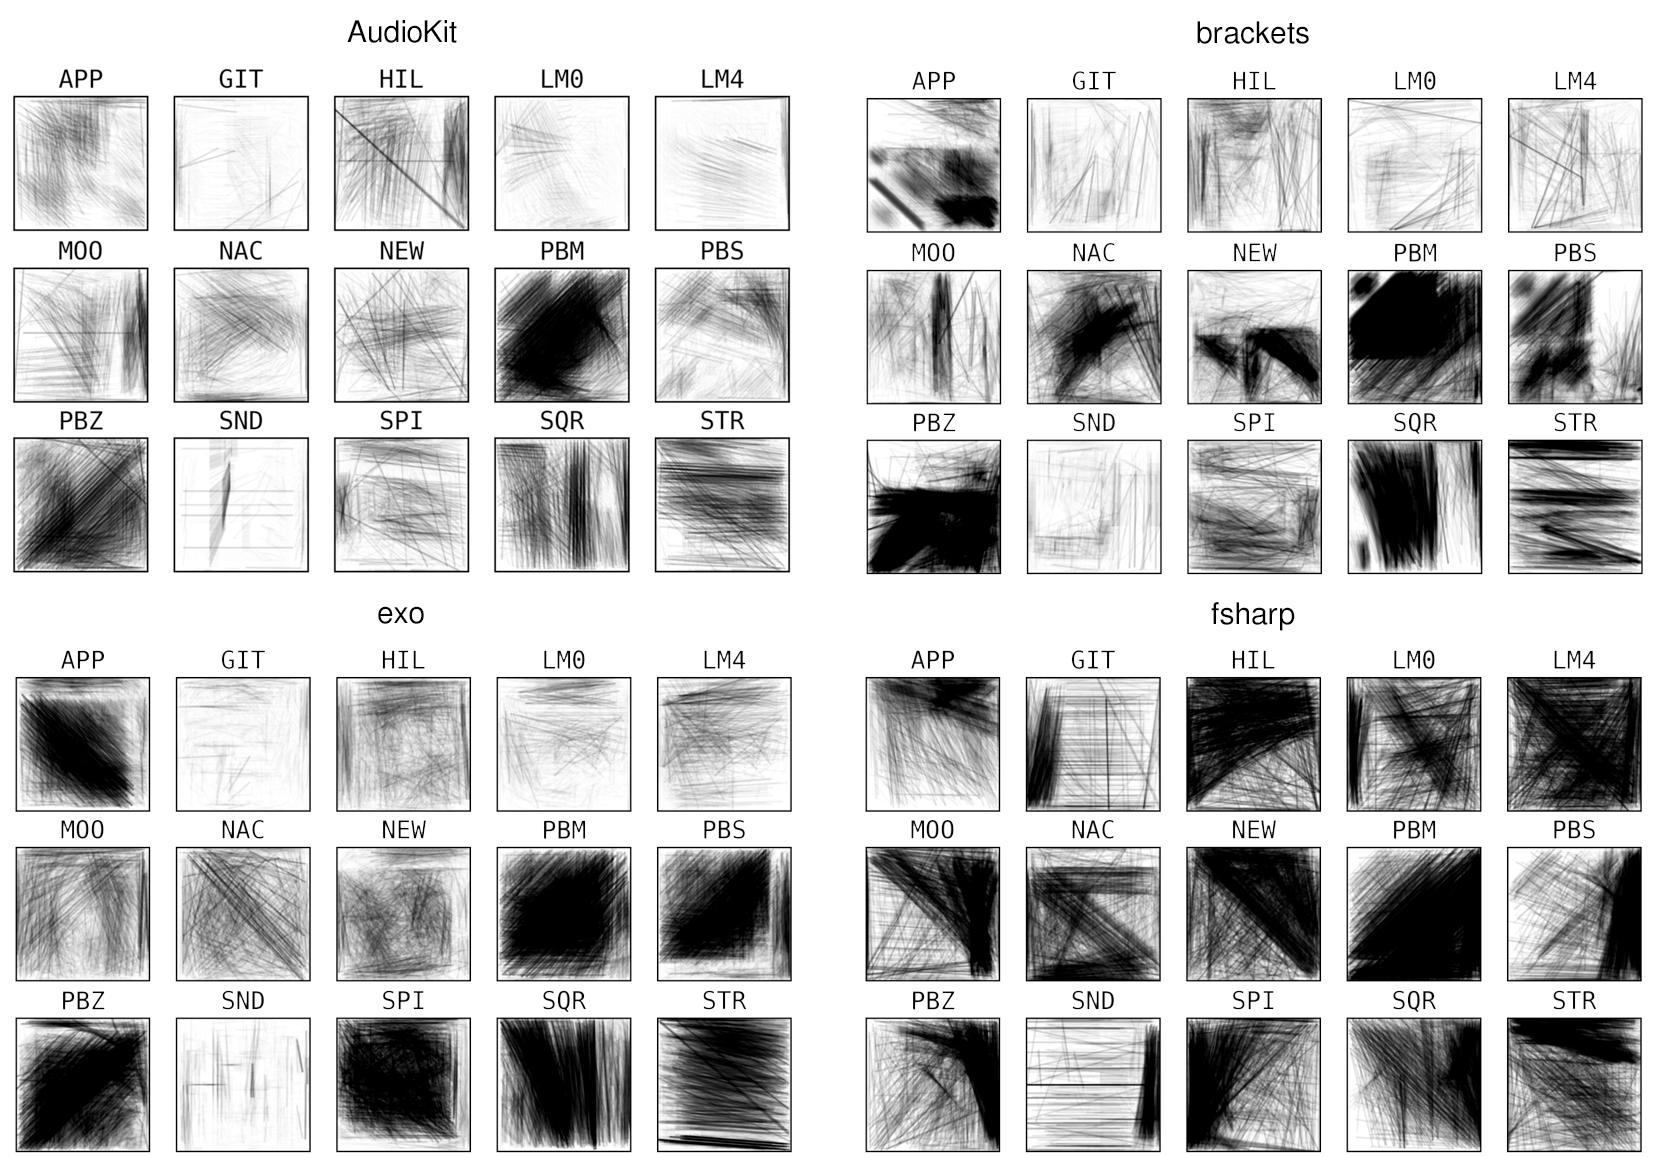
\includegraphics[width=\textwidth]{figures/treemap-algorithm/centroid-4.png}
\caption{Instability (cell center motion) patterns, all methods, \emph{AudioKit}, \emph{brackets}, \emph{exo} and \emph{fsharp} datasets.}
\label{fig:centroids}
\end{figure*}

\subsection{How do all quality metrics vary over all datasets?}
%
The experiments so far do not show the individual stability metrics (including $LD$, which can be only computed for an entire sequence), nor, for space reasons, the metrics over all 28 tested tree sequences. To get more insight in how GIT performs in these respects, we show the per-dataset average values (for $AR$ and the three stability metrics) for all tested methods, all datasets (Fig.~\ref{fig:tables}). Cells are colored using a purple (low values) to yellow (high values) colormap. We observe the following: For $AR$, APP scores consistently better for most datasets than all other tested methods. SQR reaches the highest $AR$ values, but only for a very few datasets. SND, as expected, scores overall the poorest. The remaining methods can be divided roughly into two groups, with NEW, PBM, PBS, STR, and PBZ scoring overall higher than GIT, HIL, LM0, LM4, MOO, and NAC. Concerning stability, SND scores consistently the best for all three considered metrics, and GIT, LM0, and LM4 come in the second place. This strengthens our earlier observation that GIT strikes a good balance between stability and spatial quality.

\begin{figure}[htbp!]
%\includegraphics[width=.5\textwidth]{figures/tables.png}
\includegraphics[width=.8\linewidth]{figures/treemap-algorithm/tables.png}
\caption{Average metric values for all techniques and all datasets.}
\label{fig:tables}
\end{figure}

\subsection{How to summarize GIT's quality?}
%
As noted, GIT seems to strike a good balance between spatial quality and stability. We summarize both these metrics for GIT and all other algorithms using a star plot (Fig.~\ref{fig:star-3}). The figure shows a scatterplot with $x$ mapping average stability $S$ and $y$ aspect ratio $AR$, respectively. Categorically colored points, one color per method, indicate the tested methods, attributed by their $S$ and $AR$ values over all datasets, all time steps. From each point (method), we draw lines connecting it with the $S$ and $AR$ values obtained for all the 28 tested datasets. A good algorithm has thus its `star' center placed top-right and relatively short star arms, indicating consistent quality over the entire dataset collection. We see several patterns, as follows.

At a high level, stability is roughly inversely correlated with spatial quality -- methods that score very well on one tend to score worse on the other. We see three groups of methods: APP, PBS, SQR, PBM, STR, PBZ and NEW score well on spatial quality, but poorly (except NEW) on stability. SND is the opposite outlier, scoring best on stability but clearly poorest on spatial quality. A middle group of methods (GIT, LM0, LM4, MOO, NAC, SPI, and HIL) trades well stability \emph{vs} spatial quality. Within these, GIT scores the best stability, and LM0 the best spatial quality. As such, GIT and LM0 can be considered complementary methods with respect to the stability \emph{vs} spatial quality trade-off. However, LM0 has a considerably more complex and slower implementation than GIT -- for details, we refer to~\citep{sondag17}. Separately, we see that GIT's star size (convex hull containing the lines emerging from the GIT point) is one of the smallest of all tested methods. Hence, GIT offers one of the most consistent behaviors over the entire dataset collection from all tested algorithms.

\begin{figure}[htbp!]
  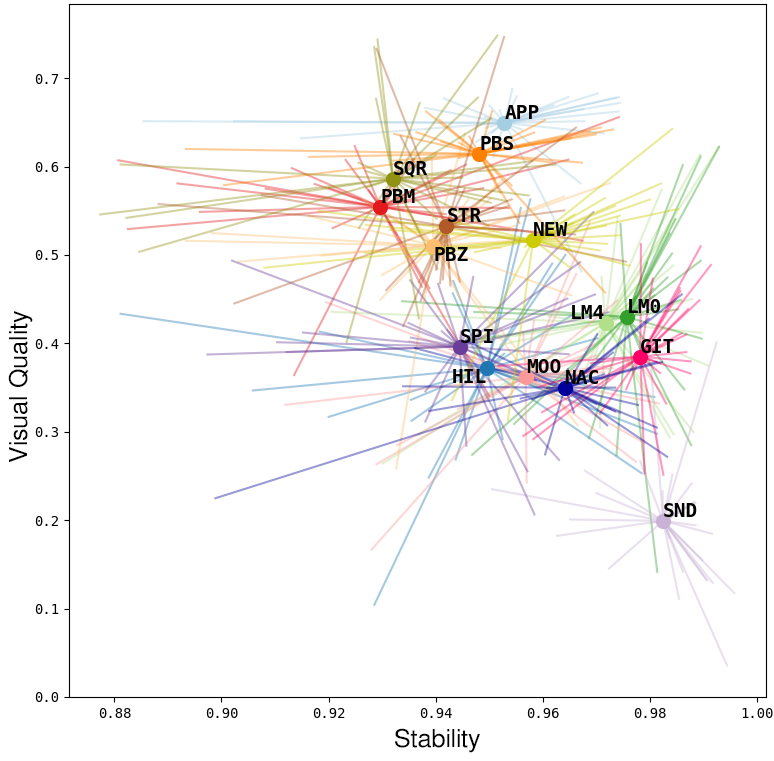
\includegraphics[width=1.0\linewidth]{figures/treemap-algorithm/star.png}
\caption{Star plot summarizing both visual quality and stability, all algorithms, all datasets.}
\label{fig:star-3}
\end{figure}

\section{Conclusion}
\label{sec:conclusion-3}
We have presented a new method for computing treemap layouts for time-dependent hierarchies. As discussed earlier, there are only a few methods in the literature that consider quality aspects pertaining to \emph{both} spatial quality and stability of such treemaps. Our contribution, in brief, is proposing a new method that takes both these quality aspects into account; and evaluating our method comprehensively on a broad dataset of 28 time-dependent hierarchies extracted from real-world dynamic dataset (software repositories), against 14 well-known treemapping methods, and using 4 quality metrics. Our results show that our new method strikes a good balance between spatial quality and stability as compared to state-of-the-art methods. Additionally, our method is simple to implement, fast, generic (with respect to the considered dynamic hierarchies), and has no hidden free parameters. More importantly, our method is an addition of a very small set of so-called \emph{stateful} methods that consider the evolution of a dynamic tree sequence when computing suitable treemaps thereof. Most existing treemapping methods are not designed to consider tree state, which arguably makes them suboptimal for handling inherently stateful datasets like dynamic trees.

Several future work directions are possible, as follows. Firstly, it is interesting to extend our evaluation to dynamic hierarchies from other domains than software evolution. This may show how much our proposal can effectively handle such more diverse datasets. Secondly, we argue that more refined quality metrics are needed (in general, for our new method but also any other treemapping methods) to capture the quality of such methods, as perceived by end users and in sync with their tasks. Finally, understanding the trade-off between the (algorithmic) reasons behind spatial quality and stability, \emph{i.e.} what to do to optimally satisfy both these requirements, is an open problem, to which we believe to have contributed to with our current work.

\newpage
